\chapter{Contributions}\label{chap:tra}

\section{Présentation de l'outil Acceleo}\label{sec:acc}

Acceleo est un générateur de code Open Source développé par \kwobeo{} et la fondation Eclipse.
\\
Acceleo permet de générer du code, à partir de modèles basés sur le framework EMF (\cf{} \cite{emf}), en mettant en œuvre l'approche Model Driven Architecture (MDA). Le générateur Acceleo est une implémentation de la norme de l'OMG pour les transformations de modèle vers texte (Model to Text : M2T \cf{} section \ref{sec:m2t}.

\subsection{Fonctionnement}

Comme la plupart des générateurs de code, Acceleo propose un système basé sur les templates : Les fichiers à générer peuvent être écrits avec des éléments statiques mêlés à des éléments dynamiques.

\subsubsection{Les Modules}

Dans Acceleo, un Module est une unité de génération amenée a être utilisée par le générateur. Un générateur est donc une agrégation de Modules.
\\
Un Module est paramétré par un ou plusieurs DSL (ndla : définir précédemment, a vérifier) afin de pouvoir proposer les fonctionnalités associées, qui permettent notamment de parcourir chaque élément du Modèle.
\\
Chaque Module est composée d'un ou plusieurs templates. Un template a pour rôle de générer du code d'après un ou plusieurs paramètres (éléments du Modèle). L'utilisation des templates est rendue très intuitive grâce au langage conçu pour Acceleo : Par défaut, le texte écrit dans un Template est recopié tel-quel dans le fichier qui sera généré en sortie. Afin d'insérer du contenu dynamique (base de la génération) dans le texte du Template, Acceleo utilise les balises \guim{\textbf{[}} (ouvrantes) et \guim{\textbf{/]}} (fermantes). Ces balisent permettent d'insérer un certain nombre d'instructions, comme la récupération d'un attribut d'un élément du Modèle, mais aussi des opérations conditionnelles ou des boucles de traitement.
\\
Par convention, chaque Module concerne un ou plusieurs aspects de la génération. Un Module peut également être dédié à la génération d'un type de fichier en particulier.

\begin{figure}[htb]
  \centering
  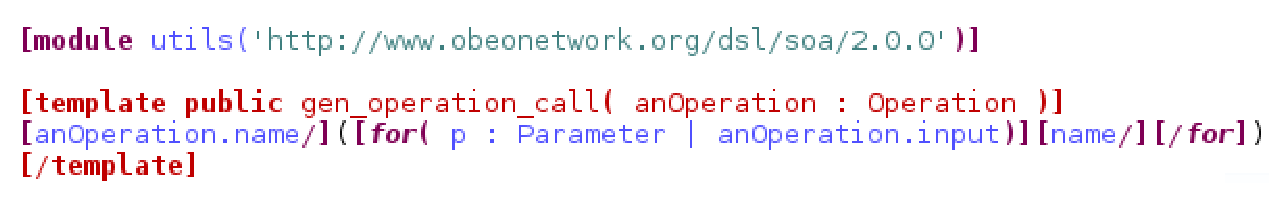
\includegraphics[scale=0.6]{img/screen_template.eps}
  \caption{Exemple de fichier Module dans Acceleo}
  \label{fig:acc_module}
\end{figure}

% Peut être une tite capture d'écran ici (Je m'en charge)

\subsubsection{Les Queries}

Les Modules permettent de décomposer la génération du code en plusieurs sous-parties réutilisables. Ils sont donc utiles pour générer un même type de contenu texte à partir de différents éléments du même type.\\
Cependant, dans certains cas, il est nécessaire d'exécuter une opération sur un élément du Modèle, comme la modification d'une chaine, ou l'accès à l'élément parent d'un élément, par exemple.\\
Les Queries interviennent alors comme un moyen de déporter ces opérations non-triviales dans une base commune. Les spécificité des Queries par rapport aux templates est que ces dernières mettent en cache leur résultat. Ainsi, si une Query est appelée deux fois avec les mêmes paramètres, celle-ci ne sera pas re-calculée et se contentera de retourner le résultat obtenu précédement. Cette fonctionnalité est donc très utile pour l'appel répétitif d'opérations (même basiques), ou le stockage de variables globales.\\
Les Queries permettent plus généralement de structure le générateur. Par convention, les générations de texte sont traitées dans des templates, tandis que les opérations plus complexes (modification de chaine, parcours d'éléments) ou répétitive sont déportées dans des Queries.

\begin{figure}[htb]
  \centering
  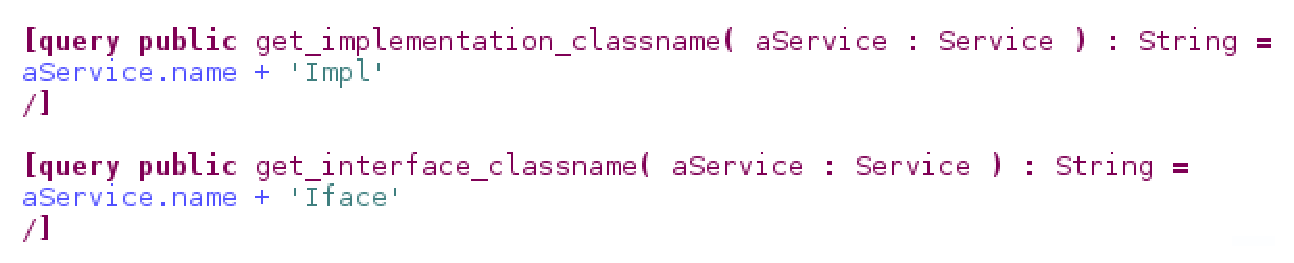
\includegraphics[scale=0.6]{img/screen_query.eps}
  \caption{Exemple de Queries dans Acceleo}
  \label{fig:acc_module}
\end{figure}

\subsubsection{Les Services}

Les Services peuvent être vus comme une extension des Queries. Là où les opérations exécutables des Query se limitent à celles d'Ocl (TODO : Aborder Ocl). Le principe des Services consiste à appeler du code Java depuis une Query via des invocations de méthodes. Cela permet d'effectuer des opérations complexes ou bien de stocker un certain nombre d'informations via du code Java. Ces informations restent récupérables depuis les templates pendant toute la durée de la génération de code.

\subsubsection{Les balises \guim{Code Utilisateur}}

Si un Générateur de Code permet aisément de transcrire la structure et la logique de fonctionnement d'un système, il est en revanche impossible d'en saisir automatiquement tous les aspects ou particularités. En d'autres termes, un code généré sera rarement complet. \kwacceleo fournit donc un système très simple permettant de définir des zones de \guim{Code Utilisateur} au sein d'un Template. Ainsi, l'utilisateur peut apporter des modifications ou ajouts dans les fichiers générés. Si ces modifications ont été effectuées à l'intérieur d'une zone \guim{Code Utilisateur}, ces dernières ne seront pas affectées si les fichiers sont générés à nouveau. De telles zones peuvent être insérée au sein d'un Template en utilisant de simples balises \guim{\textit{\textbf{[protected]}}}

% Ici un schema ?
\begin{figure}[htb]
  \centering
  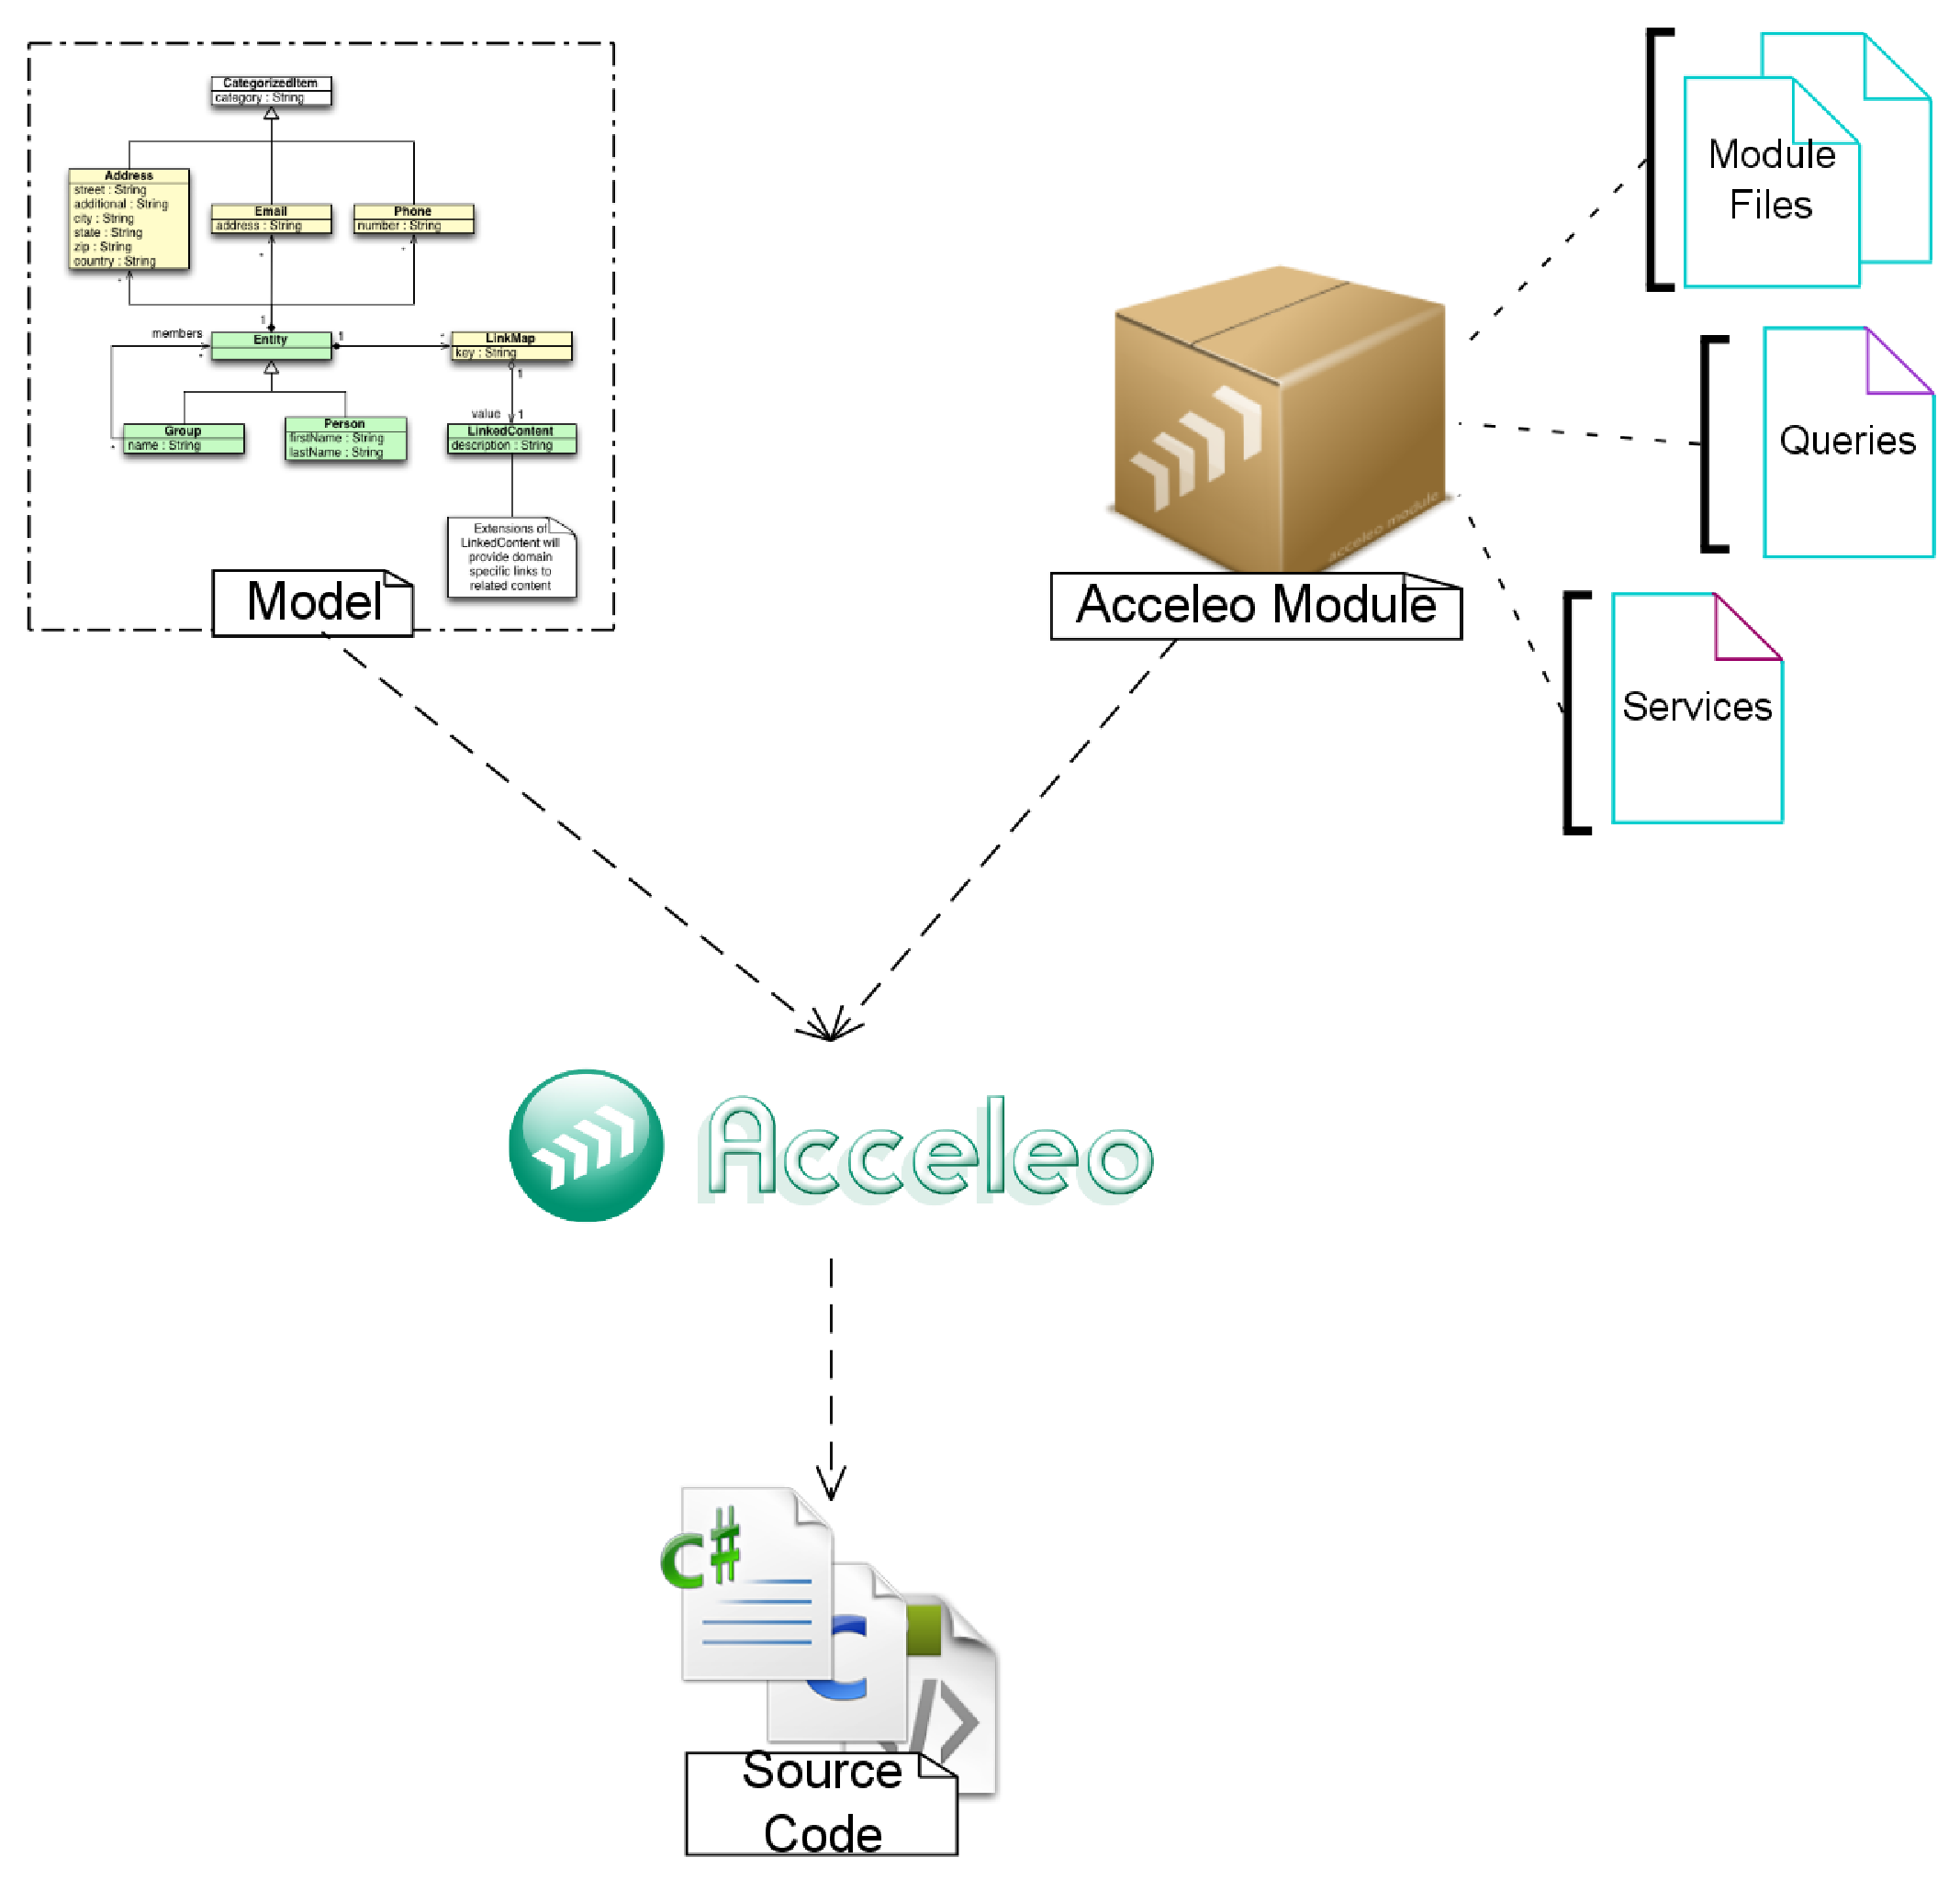
\includegraphics[scale=0.29]{img/acceleo_scheme.eps}
  \caption{Fonctionnement d'Acceleo}
  \label{fig:acceleo}
\end{figure}

%\subsection{Déploiement}
%
%Afin de gérer le déploiement des différents générateurs de %code, 

% Causer du système de menus/plugins/etc

\newpage

\section{Le Méta-Modèle Entity}\label{sub:ent}
Les Entity permettent de simplifier la gestion des données au niveau d'une application, mais aussi de faciliter la sauvegarde en base de données. Plus concrètement, ces Entity nous permettent de prendre en charge la persistance des données de notre application dans une ou plusieurs sources de données, tout en gardant les relations entre celles-ci. Ces composants établissent donc la relation entre notre application et notre bases de données.
Un méta-modèle Entity a été établie par Obeo afin de représenter la structure des Entity qui vont définir la couche métier de notre application. La figure \ref{fig:ent}  montre le méta-modèle Entity simplifié.

\begin{figure}[htb]
  \centering
  
\includegraphics[scale=.4]{img/Entity.eps}
  \caption{Méta-modèle Entity}
  \label{fig:ent}
\end{figure}

Tout modèle conforme au métamodèle "Entity" peut être constitué de plusieurs de plusieurs Bloques (blocks). Chaque bloque se compose de plusieurs Entity. Celle-ci possède un ou plusieurs attributs, et peut référencer d'autres Entity. Un attribut peut avoir une métadonnée qui peut être constituée d'une ou plusieurs annotations.   

\subsection{Gestion des entités avec \kwplay{}}
Dans la plate-forme Play, tout le code métier est porté par les objets du modèle. Celui-ci contient les données persistantes, ce qui s'accordent parfaitement avec le concept d'\kwentity.  
On peut par exemple écrire le code suivant pour manipuler une entité "Personne" :\\
// Si on voulait récupérer toutes les personnes    \\
List<Personne> personnes = Personne.find("byName","Takfarinas").fetch();  \\
Personne p1 = Personne.findById(1);  // Récupérer la personne ayant l'id 1  \\
p1.firstName = "paul";  // Modification de l'entité  \\
p1.save(); // Mise à jour dans la base de données    
         

\subsection{Conception du modèle}
Nous avons employé la simple démarche suivante : pour chaque modèle \kwplay{} on associe une entité. À ce stade, on en déduit facilement les attributs de chaque instance d'\verb+Entity+ et les instances \verb+Reference+ correspondant aux associations avec d'autres entités. \kwplay{} utilise des mécanismes d'annotation au sein de ses modèles. Ces annotations permettent notamment de donner des contraintes à des attributs. Nous avons facilement pris en compte ce concept en utilisant la classe \verb+Annotation+ mise à disposition dans les méta datas d'un \verb+Attribut+.\\
Nous avons élaboré un modèle d'entity de notre application conformément au méta-modèle que nous avons décris en dessus. Ce modèle est illustré par la figure \ref{fig:entMod} ci-dessous.

\begin{figure}[H]
  \centering
%$  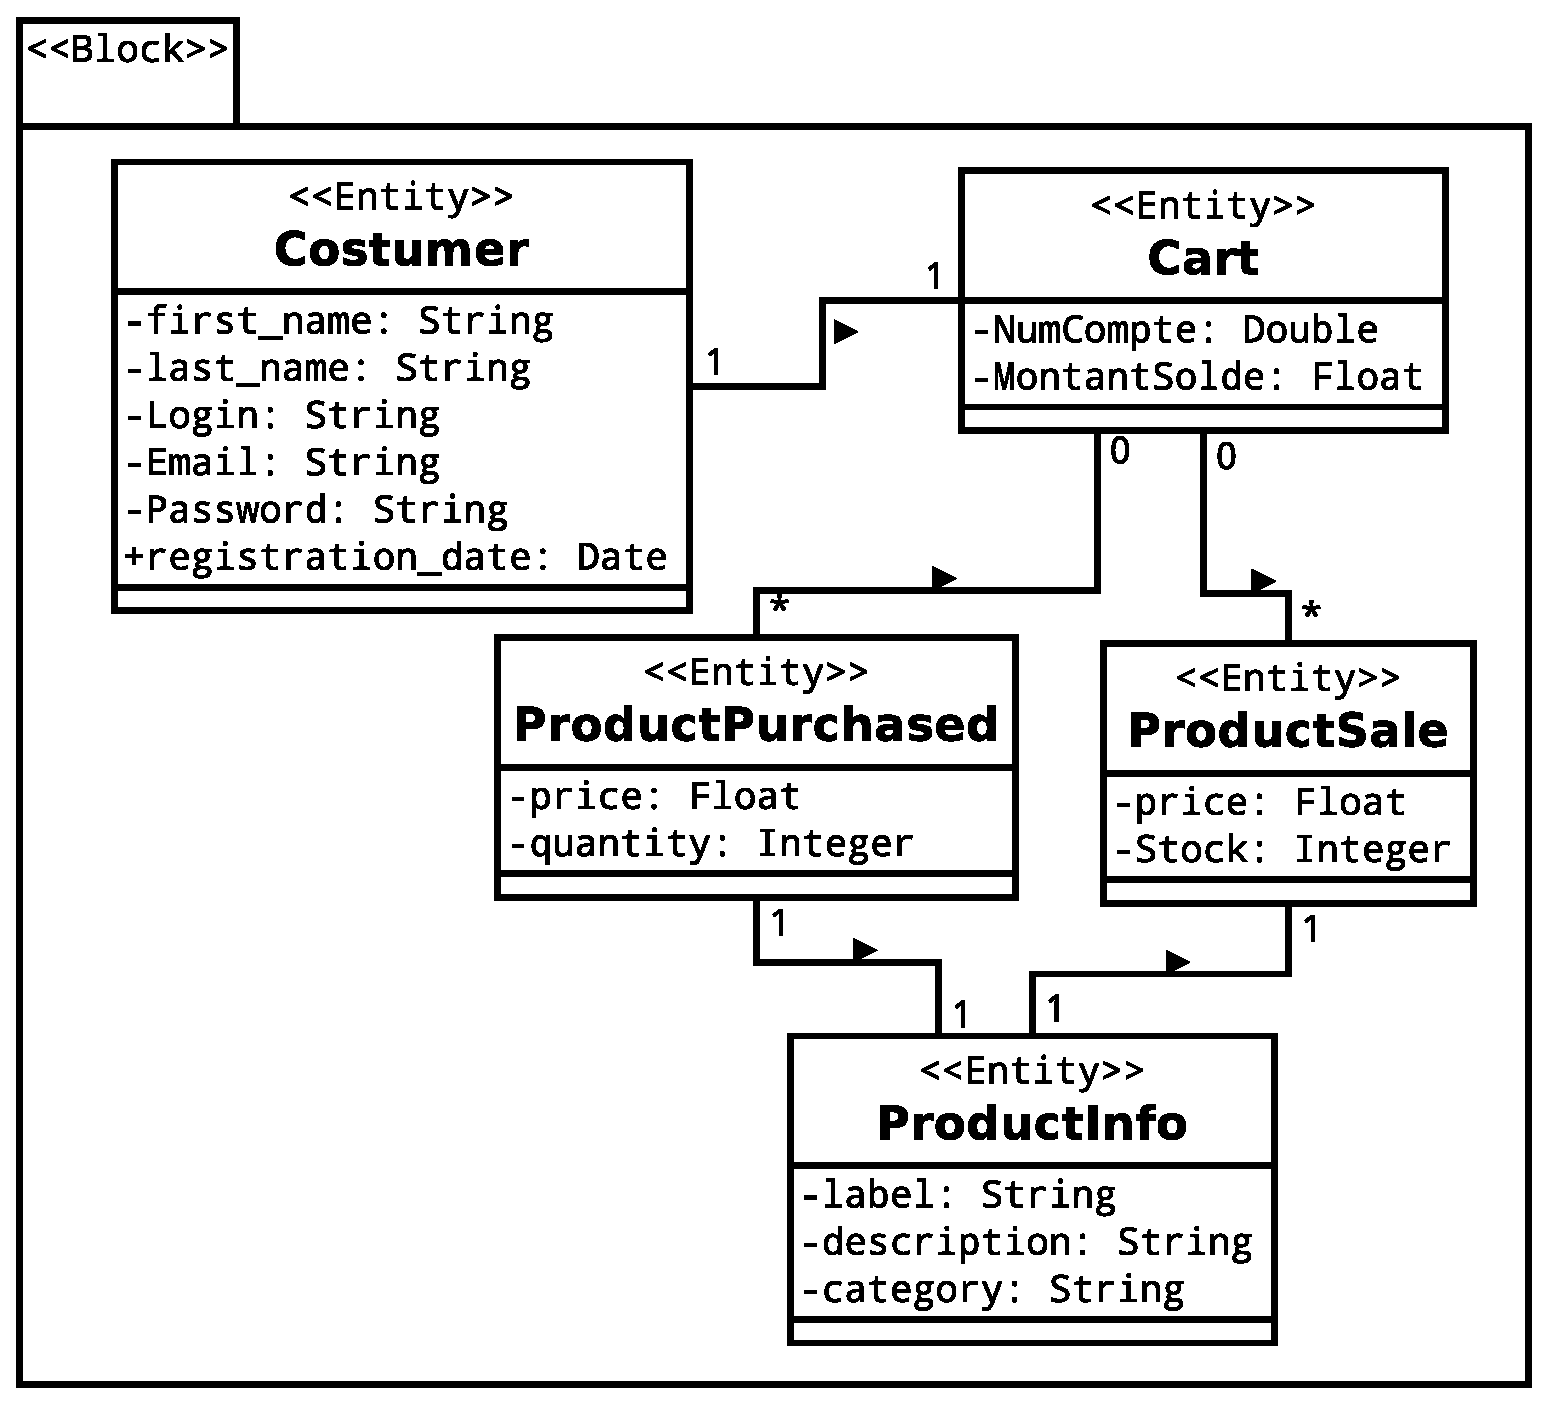
\includegraphics[scale=.4]{img/Entitymodel.eps}
  \caption{modèle Entity de l'application}
  \label{fig:entMod}
\end{figure}

Nous avons représenté un seul bloque dans notre modèle d'Entity qui va regrouper les Entity suivantes :  

\begin{itemize}
  \item[\textbullet] \textbf{Costumer} : Représente le client qui va faire l'achat sur la plate-forme
  \item[\textbullet] \textbf{ProductSale} : représente les produits mises en vente.
  \item[\textbullet]	\textbf{ProductPurchased} : représente les produits achetés par un client.
  \item[\textbullet] \textbf{ProductInfo} : contient les informations d'un produit.
  \item[\textbullet] \textbf{cart} : représente une carte de paiement reliant un client aux produits qu'il a acheté.
   
\end{itemize}

\subsection*{Génération de code Entity}





\clearpage



% LocalWords:  Entity framework Model
 
\section{SOA}\label{sub:soa}
blah bklah fdslmk blah bklah fdslmk 
\begin{figure}[htb]
  \centering
  
\includegraphics[scale=.3]{img/SOA.eps}
  \caption{Méta model SOA}
  \label{fig:soa}
\end{figure}


\section{Cinématique}
\subsection{Modélisation}
\subsubsection{Vue globale du métamodèle}
Le métamodèle est organisé autour de trois principaux packages:
\begin{itemize}
  \item View: représente les concepts liés à la définition des écrans IHM.
  \item Toolkit: représente les concepts liés à la définition des
  widgets\footnote{Elément visuel d'une interface graphique (bouton, ascenseur,
  liste déroulante, etc.)} IHM.
  \item Flow: permet d'identifier le comportement dynamique des écrans IHM.
  Le flow peut être appréhendé comme une sorte de diagramme d'activités.
\end{itemize}

\inputnp{4d_Deploiement}
